\documentclass[10pt,twocolumn,letterpaper]{article}

\usepackage{cvpr2019AuthorKit/latex/cvpr}
\usepackage{times}
\usepackage{epsfig}
\usepackage{graphicx}
\usepackage{amsmath}
\usepackage{amssymb}
\usepackage{xcolor}

% Include other packages here, before hyperref.

% If you comment hyperref and then uncomment it, you should delete
% egpaper.aux before re-running latex.  (Or just hit 'q' on the first latex
% run, let it finish, and you should be clear).
\usepackage[breaklinks=true,bookmarks=false]{hyperref}

\cvprfinalcopy % *** Uncomment this line for the final submission

\def\cvprPaperID{****} % *** Enter the CVPR Paper ID here
\def\httilde{\mbox{\tt\raisebox{-.5ex}{\symbol{126}}}}

% Pages are numbered in submission mode, and unnumbered in camera-ready
%\ifcvprfinal\pagestyle{empty}\fi
\setcounter{page}{4321}
\begin{document}

%%%%%%%%% TITLE
\title{Multi-modal task transfer learning for Vehicle Re-Identification}

\author{First Author\\
Institution1\\
Institution1 address\\
{\tt\small firstauthor@i1.org}
% For a paper whose authors are all at the same institution,
% omit the following lines up until the closing ``}''.
% Additional authors and addresses can be added with ``\and'',
% just like the second author.
% To save space, use either the email address or home page, not both
\and
Second Author\\
Institution2\\
First line of institution2 address\\
{\tt\small secondauthor@i2.org}
}

\maketitle
%\thispagestyle{empty}

%%%%%%%%% ABSTRACT
\begin{abstract}
  abstract  abstract  abstract  abstract  abstract  abstract  abstract  abstract  abstract  abstract  abstract  abstract  abstract  abstract  abstract  abstract  abstract  abstract  abstract  abstract  abstract  abstract  abstract  abstract  abstract  abstract  abstract  abstract  abstract  abstract  abstract  abstract  abstract  abstract  abstract  abstract  abstract  abstract  abstract  abstract  abstract  abstract  abstract  abstract  abstract  abstract  abstract  abstract  abstract  abstract  abstract  abstract  abstract  abstract  abstract  abstract  abstract  abstract  abstract  abstract  abstract  abstract  abstract  abstract  abstract  abstract  abstract  abstract  abstract  abstract  abstract  abstract  abstract  abstract  abstract  abstract  abstract  abstract  abstract  abstract  abstract  abstract  abstract  abstract  abstract  abstract  abstract  abstract  abstract  abstract  abstract  abstract  abstract  abstract  abstract  abstract  abstract  abstract  abstract  abstract  abstract  abstract  abstract  abstract  abstract  abstract  abstract  abstract  abstract  abstract  abstract  abstract  abstract  abstract  abstract  abstract  abstract  abstract  abstract  abstract  abstract  abstract  abstract  abstract
\end{abstract}

%%%%%%%%% BODY TEXT
\section{Introduction}

Vehicle re-identification (re-id) aims at searching vehicle instances across nonoverlapping camera views by image matching. Influenced by the recent extensive studies on person re-id \cite{gong2014re}, vehicle re-id has started to gain increasing attention in the past two years, and a number of vehicle databases and additional labelling are now available to facilitate this research \cite{liu2016vehicleid,liu2016veri,yang2015large,kanaci2018vehicle,wang2017orientation}. This area promises the potential for more flexible means for vehicle recognition and search than Automatic Number Plate Recognition (ANPR). However, vehicle re-id by visual appearance is a
challenging task due to the very similar appearance of different vehicle instances
of the same model type and colour, and a significant visual appearance variation
of the same vehicle instance in different camera views \cite{}.


Due to the fact that vehicles are rigid objects, unlike people, the orientation of the vehicle can alter very predictably the appearance of in a particular viewpoint. Hence

In this paper we propose a new mutual learning based network architecture, that aims to simulataneously learn a number of tasks, an

\section{Multi-modal Vehicle Re-identification}

In order to perform Re-ID of previously unseen query vehicles, the aim of our model is to learn an feature embedding that allows for accurate retrivals based on distance (\eg L1) from the query image representation. In order to perform this task, we utilise training data containing a number of different labels: identity class labels, vehicle orientation class labels, and landmark position labels for a number of specific keypoints. We assume two sets of training examples $\mathcal{I_1} = \{\mathbf{I_i}\}_{i=1}^N$ and $\mathcal{I}_2 = \{\mathbf{I_i}\}_{i=1}^M$, containing $N$ and $M$ training images respectively. Both training sets contain the associated identity class labels $\mathcal{Y}_1=\{y_i\}_{i=1}^N$ and $\mathcal{Y}_2=\{y_i\}_{i=1}^M$, where $y_i \in \left[1,...,N_{id}\right]$ for $N_{id}$ distinct vehicle idenities spanning the two training sets. However, in addition, $\mathcal{I}_1$ also contains orientation and landmark position labels $\mathcal{O}=\{o_i\}_{i=1}^N$ $\mathcal{L}=\{\mathbf{l_i}\}_{i=1}^N$ respectively, where $o_i \in \left[1,...,N_O\right]$ is the orientation (for $N_O$ possible orientations), and  $\mathbf{l_i}=\{\left(x_{i,1},y_{i,1}\right),...,\left(x_{i,L},y_{i,L}\right)\}$ defines the position of $L$ keypoint landmarks for the vehicle within image $\mathbf{I}_i$, which we normalise according to the image size so that $x,y \in [0,1]$

In order to perform accurate re-ID, we use this data to build a model constructed from a number of branches, each of which is tasked with learning a specific aspect of the data.

\subsection{Model Structure and Feature Learning}

\begin{figure*}
  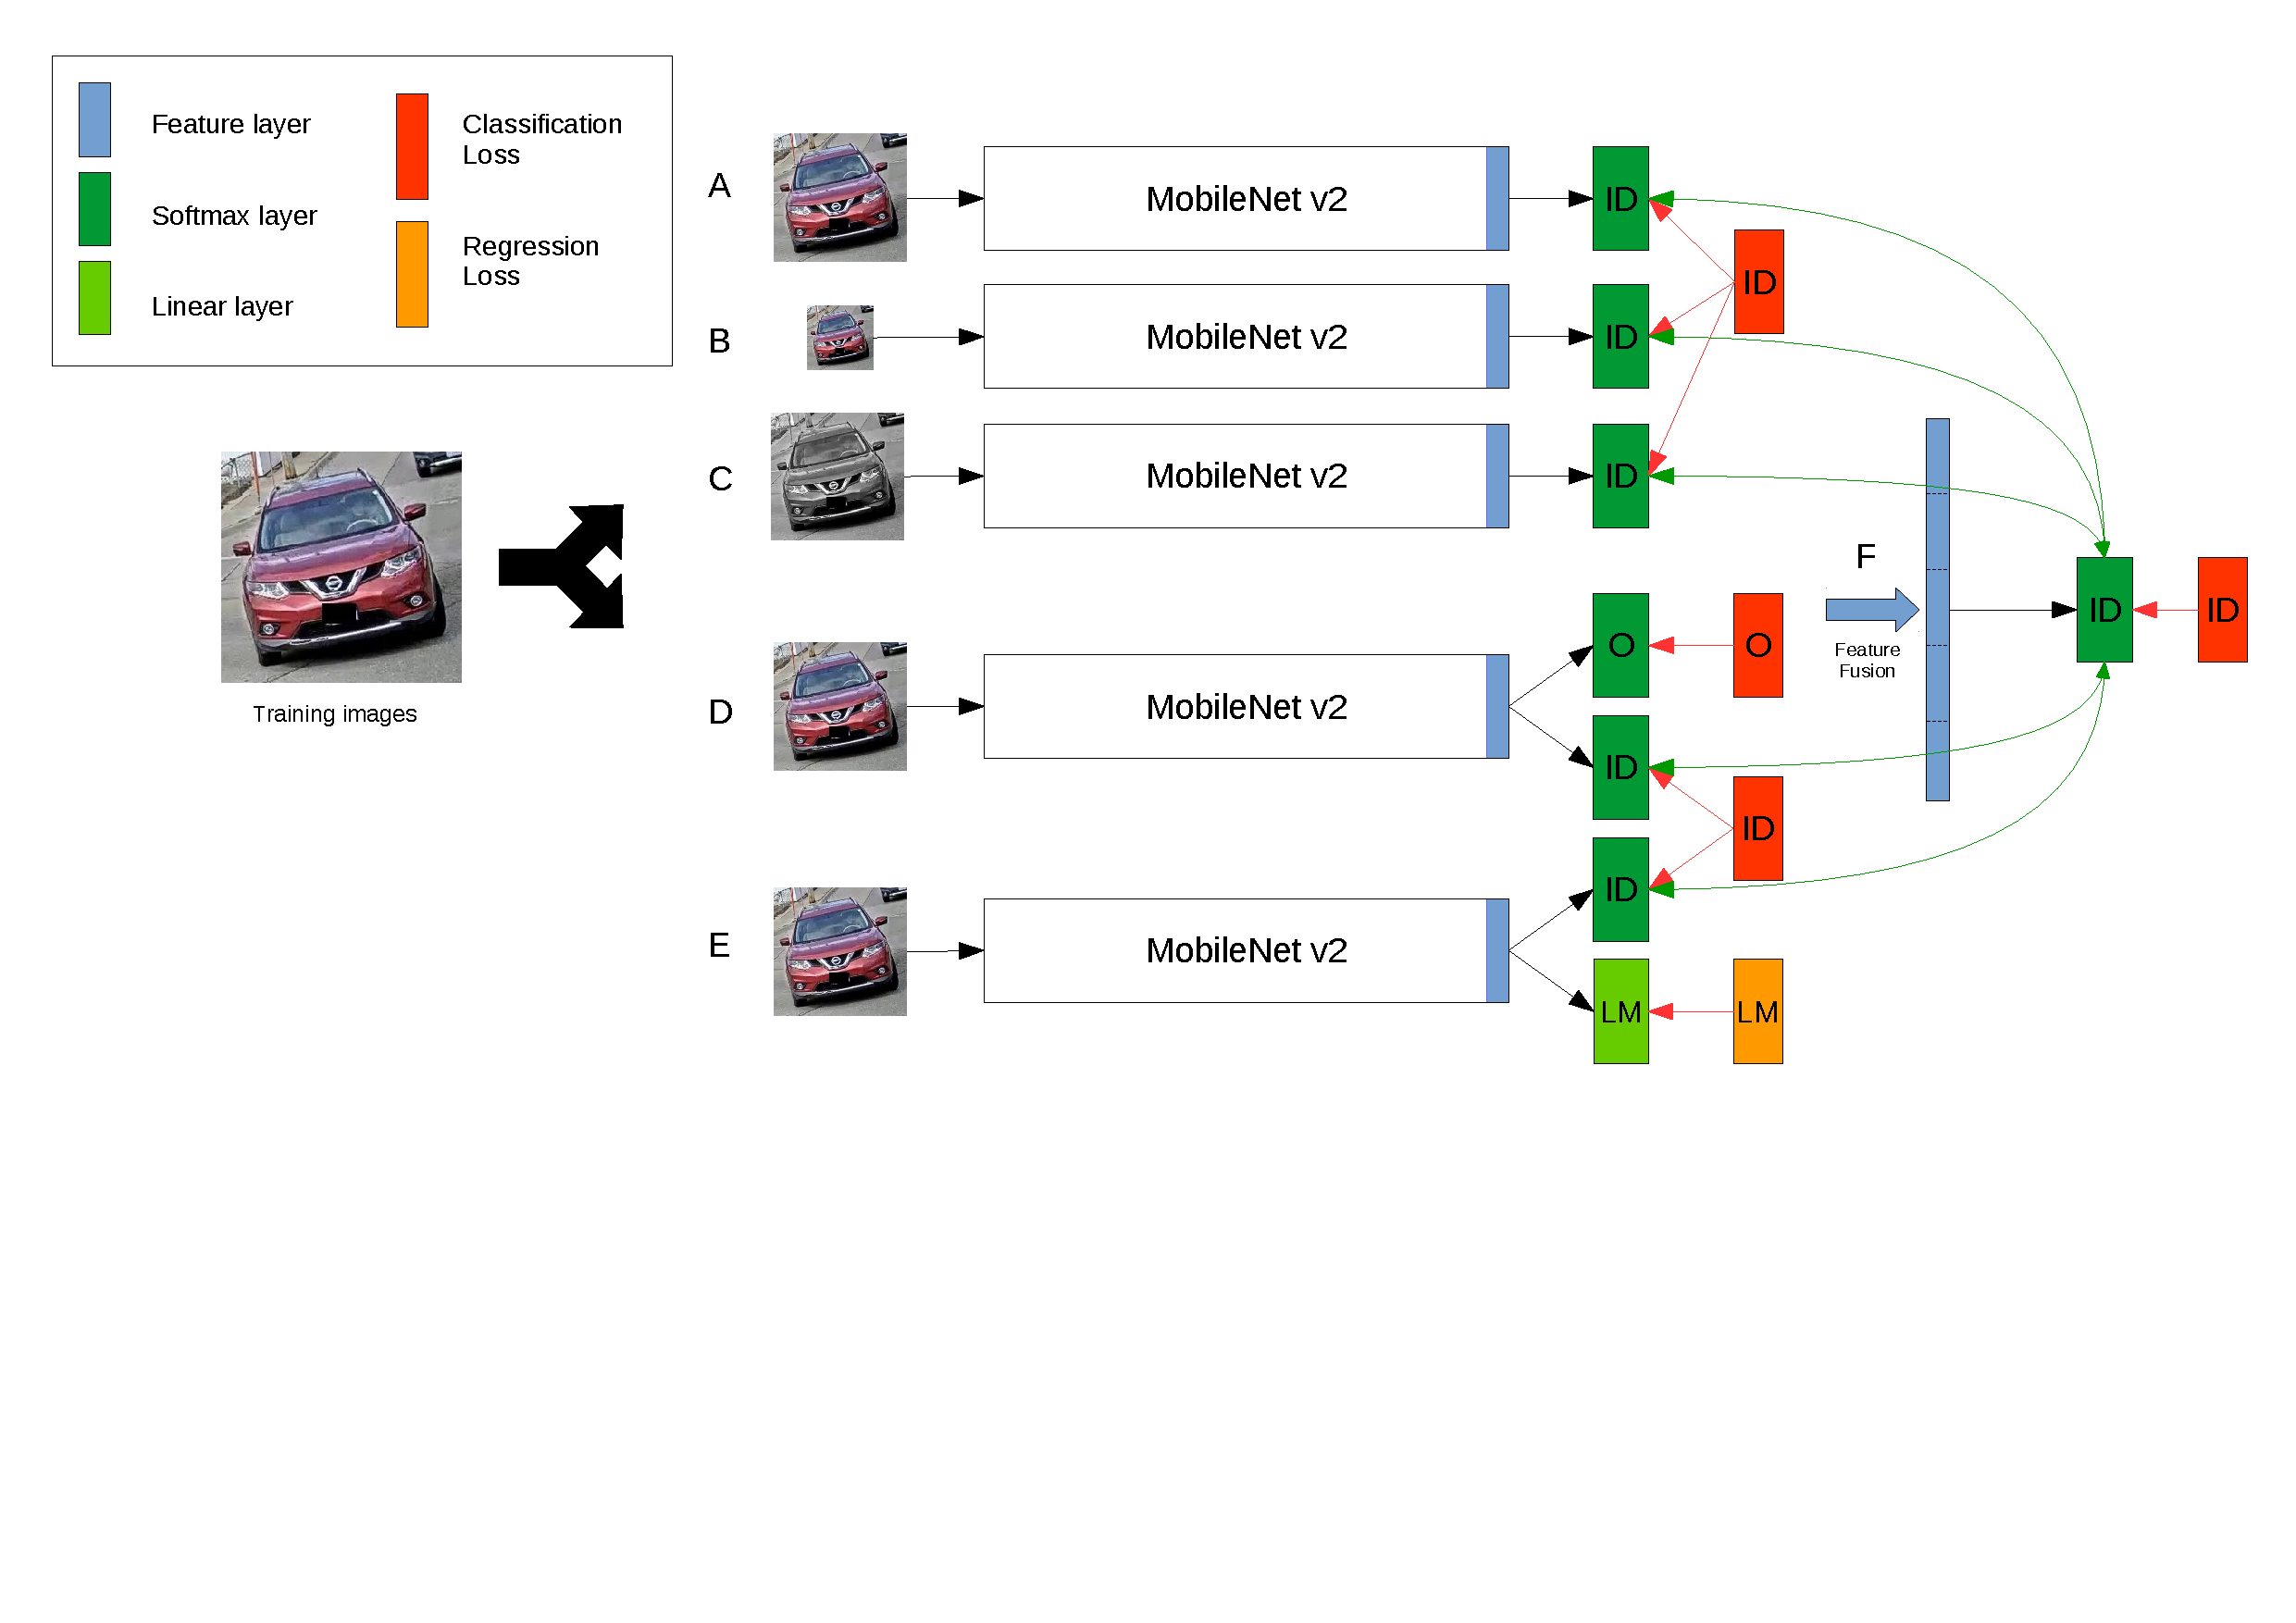
\includegraphics[width=\linewidth,trim=0cm 10cm 0cm 0cm,clip=true]{images/system_overview.pdf}
  \label{F:overview}
  \caption{An overview of our proposed model (best viewed in colour). (A) Vehicle identity branch (B) Multi-scale analysis branch (C) Grayscale analysis branch (D) Vehicle orientation branch (E) Vehicle landmark localisation branch. (F) Consensus learning through feature fusion. Feedforward signals shown in black. Hard target (groundtruth) loss propogation shown in \textcolor{red}{red}. Soft target consensus feedback loss propogation shown in \textcolor{green}{green}.}
\end{figure*}

An overview of our proposed model can be seen in Figure \ref{F:overview}. The model is composed of a number of sub-branches, each of which is simultaneously learning a representation to solve its own set of tasks. In addition, there is a single fusion branch, which allows feature selection to be performed from the entire collection of individual representations. It is the output from this branch that is taken during deployment. Each sub-branch will now be described in more detail.

\paragraph{(A) Vehicle Identity}

The root branch of our model is tasked with learning the best representation for vehicle identity discrimination, for both training sets. Here, we exploit the cross entropy classification loss function in order to train one branch to predict vehicle identity. Thus the branch calculates the softmax posterior probability of the class label $y_i$ for a given training image $\mathbf{I_i}$:
\begin{equation}
  p_i^{ID} = p(\hat{y_i} = y_i|\mathbf{I_i}) = \frac{\exp(\hat{y_i})}{\sum_{k=1}^{N_{id}}\exp(\hat{y_k})}
  \label{E:softmax_id}
\end{equation}
where $\hat{y_k} = \mathbf{w_k^Tx_i}$, $\mathbf{x_i}$ is the feature vector for image $\mathbf{I_i}$ given by final layer of the branch, and $\mathbf{w_k}$ is the prediction function parameter for identity class $\emph{k}$. The loss across a minibatch of $N_B$ images can then be computed as:
\begin{equation}
  l_{ID} = -\frac{1}{N_B} \sum_{i=1}^{N_B} \log{p_i^{ID}}
  \label{E:cross_entropy_loss}
\end{equation}

\paragraph{(B) Multi-scale Analysis}

Here we exploit the multi-scale analysis that has previously been shown to be of benefit for the task of re-identification, both for persons \cite{chen2017person} and vehicles \cite{kanaci2018vehicle}. This is done by including a branch that is trained via cross entropy loss (Eq. \ref{E:cross_entropy_loss}) to predict the class identity from a rescaled version of the input image, in a similar way to branch A.

\paragraph{(C) Identity from Grayscale Image}

In order to force the model to focus on details of the vehicles, that allow for separation of highly similar identity classes, we ensure that one branch will be unable to use colour information for distinguishing between these classes. This is simply done by giving as input only the grayscale image, and again training the branch to predict identity via the cross entropy loss.

\paragraph{(D) Vehicle Orientation}

This branch is tasked with learning a representation to simultaneously predict the identity class and the orientation class, if known. In the case where the training images do not have associated orientation labels, this branch is trained in exactly the same way as the Vehicle Identity branch outlined above. However, when orientation labels are available, both sets of labels are simultaneously employed in a joint loss function in order to optimise the branch for prediction of both identity and orientation. Again, the cross entropy loss is employed for this task. Hence, the branch calculates both Eq. (\ref{E:softmax_id}), as well as the softmax posterior probability of the orientation label $o_i$ for the image:
\begin{equation}
  p_i^{O} = p(\hat{o_i} = o_i|\mathbf{I_i}) = \frac{\exp(\hat{o_i})}{\sum_{j=1}^{N_{O}}\exp(\hat{o_j})}
\end{equation}
where this time $\hat{o_j} = \mathbf{w_j^Tx_j}$, and $\mathbf{w_j}$ is the prediction function parameter for orientation class $\emph{j}$.

The loss for this branch across the minibatch of images can then be calculated as:
\begin{equation}
  l_{O} = -\frac{1}{N_B} \sum_{i=1}^{N_B}(\log{p_i^{ID}} + \log{p_i^{O}})
\end{equation}

\paragraph{(E) Vehicle Landmark Localisation}

Vehicle landmarks are distinguishing features that must be employed in order to perform correct  re-identification of vehicles that look very similar. Hence it is crucial that our model picks up on these in its feature representation. In order to attempt to ensure this, we task one branch with simultaneously predicting the position of these landmarks (if present) as well as the identity class. As above, if no landmark labels are available in the minibatch, this branch is trained in exactly the same way as branch A. 

If landmark groundtruth labels are available, these are employed to train the branch to predict the location of the landmarks which are present, while at the same time predict identity. As a different set of landmarks are visible, depending on the orientation of the vehicle, we need to take the absence of landmarks altogether into account when training this branch. Thus, we design a loss function that only penalises the predictions for landmarks that are present in the groundtruth labels for the minibatch examples. As this is the regression problem, we also set the final layer of the branch to output with linear activation, and take the Mean Squared Error (MSE) as the basis for our custom loss function. If the landmarks were all present in every training image, we could use the standard MSE loss:
\begin{equation}
  M = \frac{1}{N_B} \sum_{j=1}^{N_L} \sum_{i=1}^{N_B} (\hat{x_{i,j}} - x_{i,j})^2 + (\hat{y_{i,j}} - y_{i,j})^2
\end{equation}
where $\hat{x_{i,j}}$ and $\hat{y_{i,j}}$ are the predicted normalised coordinates. However, we need to alter this to remove landmarks that are not present at all in the image. Hence we design a selective MSE function that only takes into account those landmarks which the groundtruth labels indicate are present in the image. Thus:
\begin{equation}
  M = \sum_{j=1}^{N_L} \frac{1}{N_{B_j}} \sum_{i \in B_j} (\hat{x_{i,j}} - x_{i,j})^2 + (\hat{y_{i,j}} - y_{i,j})^2 
\end{equation}
where $B_j$ is the subset of the minibatch examples for which landmark $j$ is present in image $\mathbf{I_i}$. Due to the nature of the landmarks, we can assume that there will be a similar number of examples in the batch that contain each landmark, hence we can approximate this as:
\begin{equation}
  M = \frac{1}{\bar{N_{B_j}}} \sum_{j=1}^{N_L}  \sum_{i \in B_j} (\hat{x_{i,j}} - x_{i,j})^2 + (\hat{y_{i,j}} - y_{i,j})^2 
\end{equation}
where $\bar{N_{B_j}}$ is the mean number of examples containing each landmark, in order to simplify the calculation. Then the full loss function for the landmark branch becomes:
\begin{equation}
  l_{LM} = M - \frac{1}{N_B} \sum_{i=1}^{N_B} \log{p_i}
\end{equation}

\paragraph{(F) Consensus Learning and Feedback}

In order to harness the benefit of all branches for the purpose of vehicle re-identification, we employ consensus learning as proposed in \cite{chen2017person} and previously harnessed for vehicle re-id in \cite{kanaci2018vehicle}. This is done via feature fusion of the final convolutional feature maps from all branches for consensus learning. As our branches are based on the MobileNet architecture, these feature maps are formed via an average pooling operation which result in feature vectors of length $1280$. Hence our fused features are of length $6400$. This is then passed to one additional identity softmax classification layer, again employed with cross entropy loss. Hence:
\begin{equation}
  p_i^C = p(\hat{y_i^C} = y_i|\mathbf{I_i}) = \frac{\exp(\hat{y_i^C})}{\sum_{k=1}^{N_{id}}\exp(\hat{y_k^C})}
\end{equation}

Additionally, we also utilise a consensus propogation mechanism, similar to the previously proposed method \cite{chen2017person,kanaci2018vehicle}. Here the consensus output is taken as 'soft targets' (as opposed to the groundtruth label 'hard targets') for the training data, and used to feedback information about the predictions made by the entire ensemble of branches. This is done concurrently with the training of the individual branches. Thie method is inspired by the idea of Knowledge Distillation (KD) \cite{hinton2015distilling}, but is different in that here we employ the combined predictions from all the 'student' branches as a \emph{virtual} teacher model, rather than utilising a pre-trainined powerful teacher model to provide the soft targets.

Specifically, the feedback mechanism employs the consensus probability predictions $P^C_i = \left[p_{i,1}^C,...,p_{i,j}^C,...,p_{i,N_{ID}}^C\right]$ given image $\mathbf{I_i}$, feeding these into the cross entropy loss between the two distributions to provide a consensus regularisation loss for the branch:
\begin{equation}
  \mathcal{H}_i = \mathcal{H}(P^C_i, P_i) = -\frac{1}{N_{ID}}\sum_{j=1}^{N_{ID}} p_j^c \log{p_j}
\end{equation}
The total consensus loss for a particular branch is then:
\begin{equation}
  l_{C} = \frac{1}{N_B} \sum_{i=1}^{N_B} \mathcal{H}_i
\end{equation}
This is added to each individual branches loss functions. In addition, this mechanism provides regularisation of the whole network by propogating all of the consensus losses back through the feature fusion layer, which also boosts the learning of the ensemble.

\subsection{Model Training}



\subsection{Vehicle Re-ID deployment}

\section{Experiments}

\section{Conclusions}

{\small
\bibliographystyle{cvpr2019AuthorKit/latex/ieee_fullname}
\bibliography{../Bibliography/reid_bibliography.bib}
}

\end{document}
